\documentclass{standalone}
% Preamble
\begin{document}

  \section{Expérimentation}
  Nous choisissons $n=4$ et le multidegré $deg=[2,2,2,2]$. Le système polynômial s'écrit
  \begin{align}
  f_1 & =
  -x_0^2x_1^2x_2^2 - x_0x_1x_2^2 + x_0x_2^2x_3 - x_1^2x_2 + x_1x_3^2 - x_0^2 + x_1x_2 - x_1 - 1, \nonumber\\
  f_2 & =
   -x_1^2x_2^2x_3^2 - x_0^2x_2^2x_3 - x_0x_1x_2x_3^2 + x_0^2x_2 - x_0x_1x_2 + x_1^2x_3 + x_0x_1 - x_1x_2 - 1, \nonumber\\
   f_3 & =
   x_0x_1^2x_2^2x_3^2 + x_0^2x_2^2x_3 - x_0^2x_1x_3^2 + x_0^2x_3^2 - x_0x_1 + 1, \nonumber\\
   f_4 & =
   -x_0^2x_1^2x_2^2x_3^2 - x_0^2x_1x_3^2 - x_0x_2^2x_3^2 - x_1x_2^2 + x_1^2x_3 - x_1^2 - x_1x_3] \nonumber\\
   \end{align}

  La matrice de Bezout $B(1)$ est de taille $384$,
   \begin{center}
  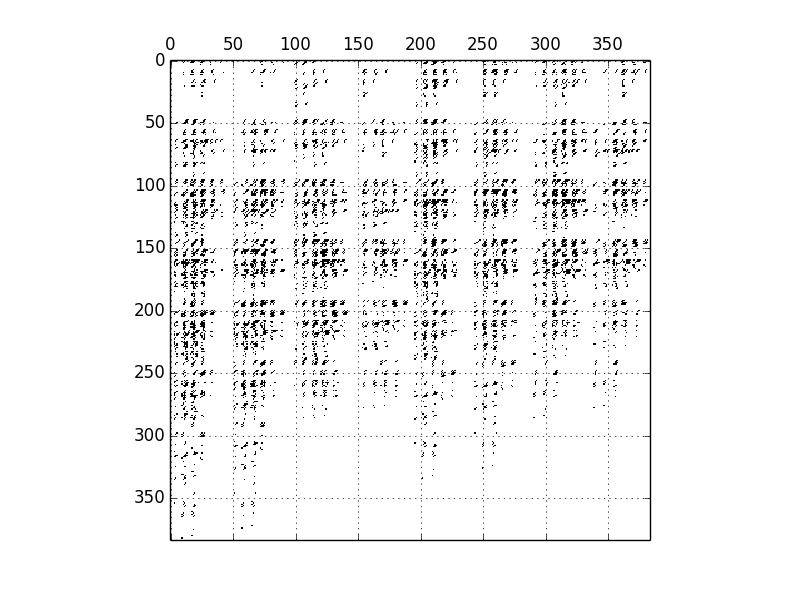
\includegraphics[width=8cm]{../png/B0.png}
  \end{center}


  En permutant lignes et colonnes on obtient une matrice bloc-triangulaire supérieure
   \begin{center}
  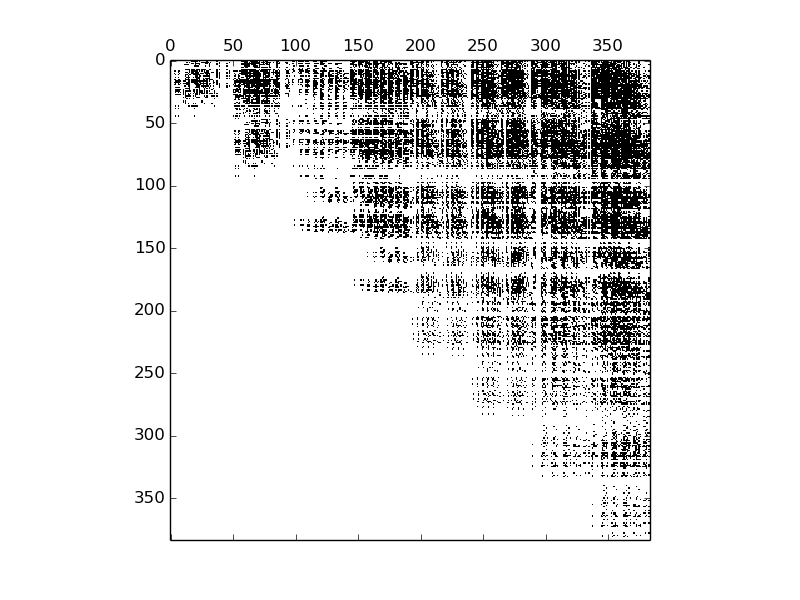
\includegraphics[width=8cm]{../png/B0_tri.png}
  \end{center}
  dont on peut calculer le noyau facilement. On trouve que rang de $B(1)$ vaut $253$.
  Une fois le processus de réduction terminé on obtient des matrices $B(1), B(x_j), j=1,\cdots,n$ de même taille, $B(1)$ étant inversible. On trouve que la dimension de $A$ est $253$. Les matrices compagnon $X_j = B(x_j)B(1)^{-1}$ fournissent alors les racines du système polynômial. Pour chacune des racines obtenues nous vérifions sa qualité en lui appliquant les polynômes $f_i, i=1,\cdots,n$ puis on représente en graphique semi-logarithmique la  valeur absolue du résultat
   \begin{center}
  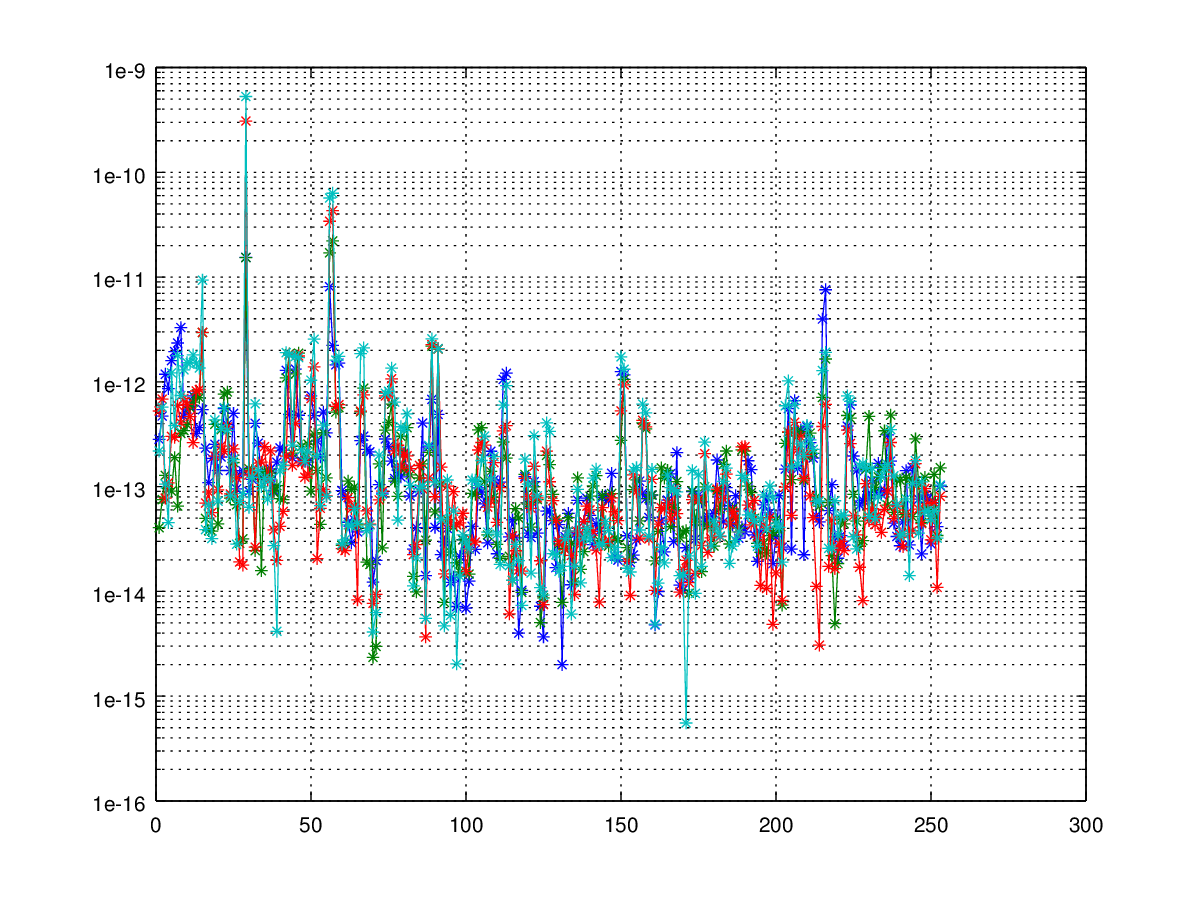
\includegraphics[height=10cm, width=18cm]{../png/f_rac.png}
  \end{center}
  Les mêmes résultats représentés sous forme d'histogramme
   \begin{center}
  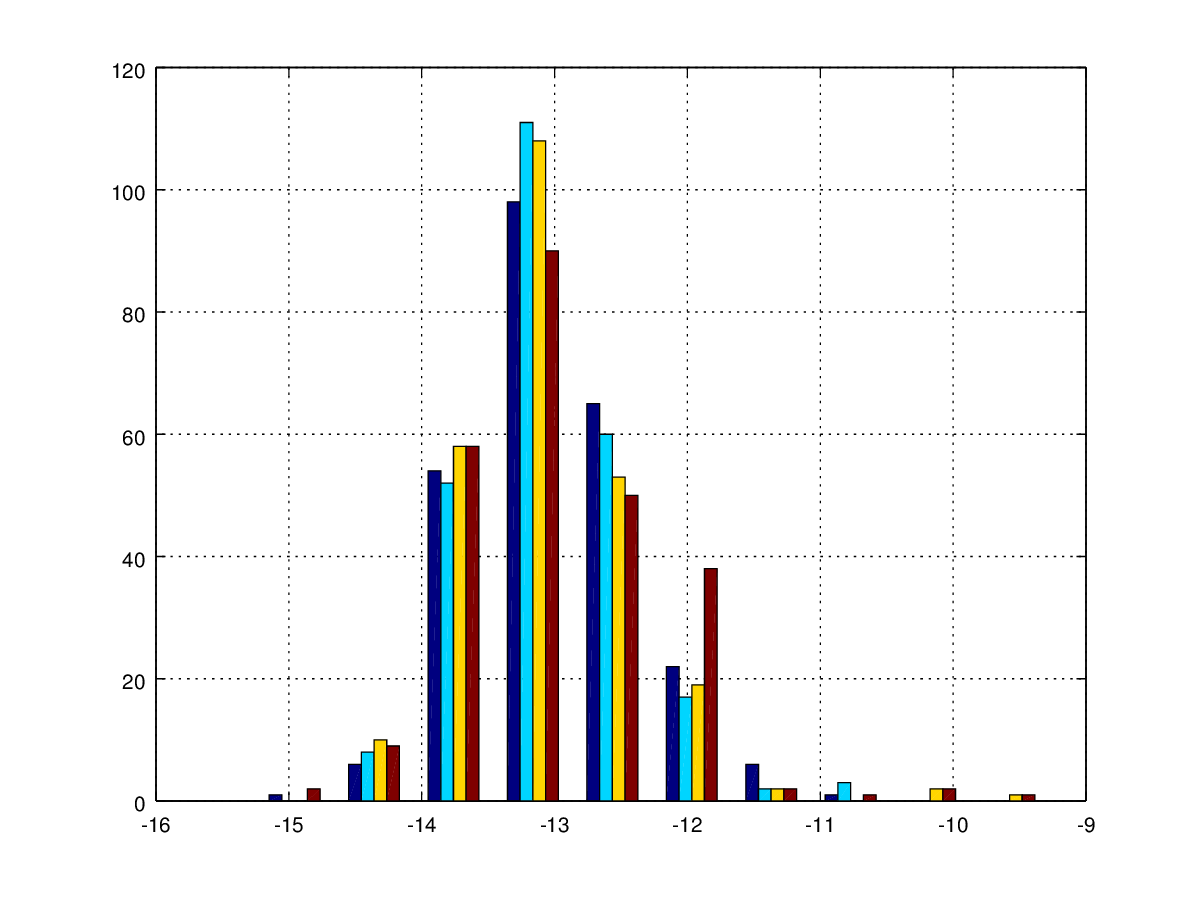
\includegraphics[height=10cm, width=18cm]{../png/f_rac_hist.png}
  \end{center}

  Dans cet exemple nous voyons que la qualité est excellente pour toutes les racines.

\end{document}
